\documentclass[12pt,a4paper]{article}
\usepackage{tabularx}
\usepackage{booktabs}
\usepackage{longtable}
\usepackage{ltxtable}
\usepackage[latin1]{inputenc}
\usepackage{amssymb}
\usepackage[]{graphicx,rotating}
\usepackage[T1]{fontenc}
\usepackage{parskip}
\usepackage{listings}
\usepackage{natbib}
\usepackage[official]{eurosym}
\usepackage{mathrsfs}
\usepackage{amsmath}
\usepackage{verbatim}
\usepackage[usenames,dvipsnames]{color}     %for R colors and formatting

\usepackage[left=3cm, right=2.5cm, top=2.5cm]{geometry}

\pagestyle{empty}
\parindent 0cm
\renewcommand{\baselinestretch}{1}
\newcommand{\bs}{\boldsymbol}
\renewcommand{\familydefault}{cmr}
\pdfminorversion=7
\bibliographystyle{agsm}

\lstset{ %for R colors and formatting
  language=R,                     % the language of the code
  basicstyle=\scriptsize\ttfa
mily, % the size of the fonts that are used for the code
  numbers=left,                   % where to put the line-numbers
  numberstyle=\scriptsize\color{Blue},  % the style that is used for the line-numbers
  stepnumber=1,                   % the step between two line-numbers. If it is 1, each line
                                  % will be numbered
  numbersep=5pt,                  % how far the line-numbers are from the code
  backgroundcolor=\color{white},  % choose the background color. You must add \usepackage{color}
  showspaces=false,               % show spaces adding particular underscores
  showstringspaces=false,         % underline spaces within strings
  showtabs=false,                 % show tabs within strings adding particular underscores
  frame=single,                   % adds a frame around the code
  rulecolor=\color{black},        % if not set, the frame-color may be changed on line-breaks within not-black text (e.g. commens (green here))
  tabsize=2,                      % sets default tabsize to 2 spaces
  captionpos=b,                   % sets the caption-position to bottom
  breaklines=true,                % sets automatic line breaking
  breakatwhitespace=false,        % sets if automatic breaks should only happen at whitespace
  keywordstyle=\color{RoyalBlue},      % keyword style
  commentstyle=\color{YellowGreen},   % comment style
  stringstyle=\color{ForestGreen}      % string literal style
} 

\begin{document}

\begin{center}
% \vspace*{1cm}
 
\includegraphics[width=0.35\textwidth]{GU-Logo-blau-CMYK.eps} \vspace{2cm}
  
  {\Large{\bf Estimating Profit-optimal Nash Equilibrium Market Shares and Prices for the Beer Market}} \medskip

  {\Large{Hierarchical Bayesian MNL Models in a Dynamic Market Environment}} \vspace{0.5cm}

  Term Paper \\\vspace{2cm}
  submitted to \\\vspace{0.5cm}
  \textbf{Prof. Dr. Thomas Otter} \\\vspace{0.5cm}
  Goethe University Frankfurt am Main \\
  School of Business and Economics \\
  Chair of Services Marketing \vspace{2cm}
  
  by \\\vspace{0.5cm}
  \textbf{Lukas J\"urgensmeier} \\
  (Mat.-Nr.: 6904281) \\
  
  \bigskip

  in partial fulfillment of the requirements of the lecture \medskip

 {\bf Customer Satisfaction and Consumer Choice} \\
  Summer Semester 2019\\
  \medskip

  July 23, 2019
  
\end{center}


\pagebreak
\pagestyle{plain}
\pagenumbering{Roman}
\tableofcontents
\pagebreak
\listoffigures
\pagebreak
\listoftables
\newpage
\setcounter{page}{2}
\pagenumbering{arabic}
\setlength{\baselineskip}{1.5\baselineskip}
\pagestyle{plain}


\section{Contextual Introduction to the Beer Market} \label{sec_intro}
\begin{itemize}
\item Beer market description: Find market study that describes competitive situation
\item Prices, Competition, Profits, Marginal Costs
\item Recent developments in the beer market (market power of few breweries)
\item Is it the Spanish beer market?
\end{itemize}

\section{Motivation of the Analytical Model} \label{sec_motivation}
Historically, marketing research has heavily relied on Conjoint Analysis.
It is a tool to measure consumers' preferences in a more realistic way by asking them to choose between different products that imply trade-offs.
This is a method to derive consumers' preferences in a more credible way than to ask them which brand or feature they prefer,
since this often yields trivial results\footnote{i.e. preferring the cheap vs. the expensive good or valuing the better quality good more than the low quality product.}.
Choice-based conjoint data enables researchers to calculate counterfactual scenarios, such as what happens to a company's market share if a competitor changes its price.
To analyze choice-based conjoint data, market research has focused on the Multinomial Logit (MNL) Model.
Unfortunately, the MNL model is based on two strong assumptions.
First, choices should be independent of irrelevant alternatives (IIA).
This means that consumers' choices are not influenced by the presence or absence of another, supposedly irrelevant other choice option.
However, numerous examples have been constructed to easily show that this assumption is often violated, most famously the blue and red bus example by \cite{mcfaddenConditionalLogitAnalysis1973}.
Especially for substitute products, this assumtion therefore does not hold. 
Modeling very similar choices with a traditional MNL model is hence not desirable.
The second strong assumption that is required for MNL estimation is homogeneity in preferences across consumers.
This implies that consumers' preferences---expressed by the beta estimates---are identical, which does not hold in reality. 

Literature has acknowledged those violations and proposed the heterogeneous MNL, a more flexible model that relaxes the IIA assumption \citep{steckelHeterogeneousConditionalLogit1988}.
As a remedy to the second critical assumption's violation, hierarchical MNL models allow for differences in preferences by modeling individual MNL models for every individual customer.

When taking the derived beta coefficients from this hierarchical MNL model to simulate individual choices as well as aggregate market outcomes and equilibrium prices,
the standard approach was to assume that all prices in the choice set were within the consumer's unobserved budget.
\cite{pachaliPerilsIgnoringBudget2017} argue that this simplification leads to a serious over-estimation of equilibrium prices.
They claim that it still holds if priors such as sign constraints are included and reasonably specified in the estimation such as in \cite{sonnierHeterogeneityDistributionsWillingnesstopay2007} and \cite{allenbyEconomicValuationProduct2014}.
Instead of "cleaning" the data until derived estimates mirror the desired price ranges, this paper follows \cite{pachaliPerilsIgnoringBudget2017}
and applies a hierarchical Bayes model which is capable of inferring previously unobserved budgets, additionally to sign constraints for $\beta_{price}$.
To that matter, the present study applies the indirect utility model by \cite{berryAutomobilePricesMarket1995}.
It is superior to the price screening model proposed by \cite{gilbrideChoiceModelConjunctive2004},
since its models a continuous choice probability dependent on price.
Logit choice probabilities need to be continuous at every draw in order to derive a pure-strategy Nash equilibrium \citep{morrowFixedPointApproachesComputing2011a, pachaliPerilsIgnoringBudget2017}.

Concluding this section, the analytical model implemented in this study addresses three serious shortcomings of most common methods to conduct a market simulation and derive profit-maximizing prices.
It relaxes the IIA assumption, allows for heterogeneous individual-level consumer preferences, and infers previously unobserved budgets.
Those three model specifications are believed to yield more realistic and less biased estimates \citep{chandukalaChoiceModelsMarketing2008, pachaliPerilsIgnoringBudget2017}.


\section{Exogenous Variables and Expected Relationships}

While the previous section motivated the analytical model and introduced model extensions to relax unrealistic assumptions,
this part introduces the empirical application of those tools.
This paper analyzes a choice-based conjoint data set for choices among different beer brands obtained by the market research institute Kantar TNS.
The data set recorded preferences for canned beer presumably in the Spanish market.
 $N=407$ respondents participated in the study and choose among $p=10$ alternatives per choice task (nine beer brands and one outside option).
Every participant performed $t=15$ choice tasks. In total, 15 distinct beer brands and one outside alternative were included in the study,
while the subjects were only presented with a subset of $p$ alternatives, always including the outside choice.
The data set consists multiple brands of the same brewery---four Amstel beers and two Estrella and Mahou beers each.
The remaining seven beer brands based on their brand names are assumed to belong to different companies.
Additionally to the beers' brand names, the price was displayed to the subjects, which ranged from 0.22 to 0.74\euro.

Consistent with economic theory, there should be a negative relationship between price and demand.
The less competition and hence more market power is present, the higher should be the prices, which should come with less demand for beer.
Since demand is measured in relative market share in this model, this means a decrease in the inside goods' shares and an increase in the outside option (i.e. consumers drop out of the market and do not purchase any product).
Besides price and market share, profit is the most important metric that is optimized by the individual players in the market.
Though there is a clear intuition how prices and market shares develop dependent on the competitive scenario, no trivial statement can be made about profits.
With higher prices comes usually a lower market share---thus we cannot tell a priori which effect should have a stronger impact on profits.

Profit will then be used to calculate the producer surplus before and after the Heineken--Amstel merger.
This metric will then be used to assess whether there is any incremental profit to this transaction.
While the next section introduces the underlying analytical model and its result, the detailed market simulation outcomes can be found in section \ref{sec_marketsim}.


\section{Model Description and Results}

Based on the motivation for the analytical model described in section \ref{sec_motivation}, this section first discusses the implemented model and then presents its results.
This study uses a heterogeneous MNL model and utilizes hierarchical Bayes methods to generate the individual-level beta coefficients and the specification of the prior distribution.
Thanks to that method, every consumer's preferences are modeled with an individual MNL model.
However, since every participant only recorded $t=15$ choice tasks, there are not enough observations to reliably estimate such a model.
That is why this study uses Bayesian estimation with Markov Chain Monte Carlo (MCMC) to sample the individual-level betas and estimate the parameters for the prior distribution.

Those beta coefficients are a measure of customer preferences---a higher beta translates to a higher preference for a product, while a negative value implies dis-utility from that good for the consumer.
The distribution of betas can then be used to compute market shares either based on posterior means, the posterior of the hierarchical prior, or the lower-level non-smooth model \citep{pachaliHowGeneralizeHierarchical2017}.
This paper makes use of the latter, since the first two methods have serious shortcomings and the latter combines the advantages from both methods.
Using the posterior means as an estimate for beta ignores posterior uncertainty and focuses too much on the middle of the market.
Optimal products will therefore tend to concentrate around the mean preferences without much differentiation between brands because it underestimates the preference heterogeneity in the population.
The second method---drawing from the hierarchical prior relies too much on the assumptions about the distributional parameters. 
According to \cite{pachaliHowGeneralizeHierarchical2017}, the lower-level non-smooth method generally outperforms the first two approaches and has more desirable characteristics.

While most market simulations do not account for consumer's budget, this study uses a heterogeneous MNL model with BLP-type indirect utility \citep{berryAutomobilePricesMarket1995}, that accounts for budgets that are inferred from choices and the minimum and maximum price chosen as proposed by \cite{pachaliPerilsIgnoringBudget2017}.
Since the probability function from this model is differentiable, one can use the derivatives-based fixed point approach for a relatively quick estimation \citep{morrowFixedPointApproachesComputing2011a}.

The implemented model constrains the beta coefficients for price and budget.
Both are restricted to positive values only, which makes the model much more realistic.
Usually one would assume the price coefficients to be negative only, however in the BLP-type specification there is a reward for not using up the entire budget. Hence, $\beta_{price}$ must be positive \citep{pachaliPerilsIgnoringBudget2017}.
In some cases, it makes sense to additionally impose ordinal constraints on the betas among brands.
This would be beneficial if there was a clear and strict preference for individual specifications of the products in question (i.e. a higher quality ceteris paribus is always more desirable).
For this particular beer data set, this cannot reasonably be justified, since there is no objective order of beers.

This part described the implemented heterogeneous MNL model with BLP-type indirect utility.
The remainder of this section focuses on the model results and specifically discusses the estimated distributions of the beta coefficients.
To estimate the betas, the MCMC routine ran for 100,000 iterations, while keeping every $15^{th}$ draw.
This lead to the loglikelihood values displayed in figure \ref{fig_mcmc}.
After removing the first 3,100 values as burn-in one can assume from a visual inspection that the algorithm converged---the time series appears to be stationary in figure \ref{fig_mcmc_burnin}.

\begin{figure}[ht]
	\centering
  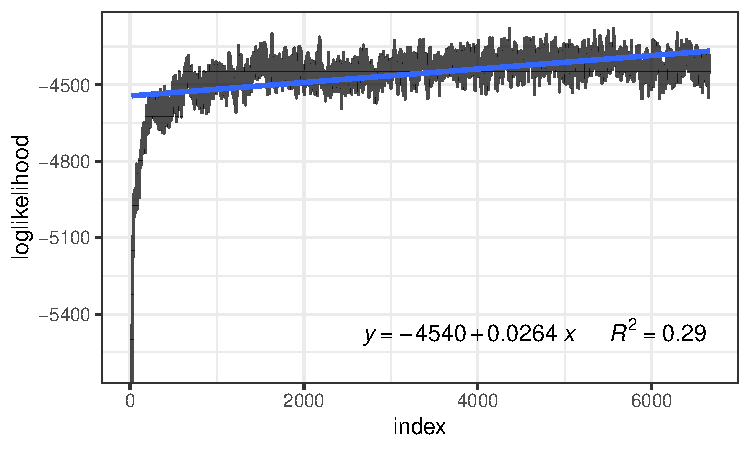
\includegraphics[scale = 0.8]{figures/mcmc_before_burnin_fitted.pdf}
	\caption{Loglikelihood values of the MCMC routine with 100,000 iterations, keeping every 15\textsuperscript{th} value}
	\label{fig_mcmc}
\end{figure}

\begin{figure}[ht]
	\centering
  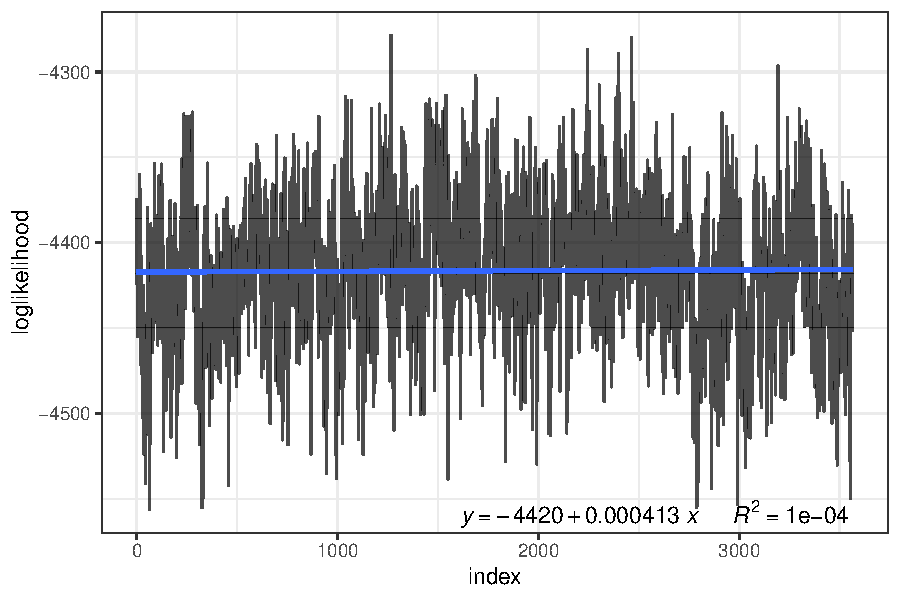
\includegraphics[scale = 0.7]{figures/mcmc_after_burnin_fitted.pdf}
	\caption{Loglikelihood values of the MCMC routine, after removing the first 3,100 observations}
	\label{fig_mcmc_burnin}
\end{figure}

The model yields the distribution of betas for all 15 brands as well as for budget and price.
Since the thorough analysis of 17 coefficients would be beyond the scope of this paper, only five presumably interesting brands\footnote{Amstel Clasica Lata, Amstel Extra Lata, Estrella Damm Lata, Estrella Galicia Lata and Heineken (all 33 cl cans)} were analyzed in detail.
The results for the entire data set can be found in the appendix in figures \ref{fig_corr_all} and \ref{fig_hist_all}.
A beta distribution with more probability mass in the positive domain of the density plot relative to others indicates that this brand is more preferred by the average customer.
Looking at the density plot for the beta coefficients of the five select beers (figure \ref{fig_dens_five}), there are some interesting differences in preferences:
First, Heineken has the highest mean and its distribution is visibly shifted to the right, compared to the other brands.
This indicates a higher preference for Heineken given identical prices for the average customer.
Secondly, both Estrella brands have less variant beta distributions, which hints at a less heterogeneous consumer segment.
On the other hand, both Amstel beers are characterized by high variance distributions with a considerable and highest relative area under the curve in the negative domain, compared to the Estrella and Heineken beers.
That means that Amstel is for many consumers the least preferred beer in this subset and even comes with dis-utility ($\beta_{i}<0$) for those.

\begin{figure}[ht]
	\centering
  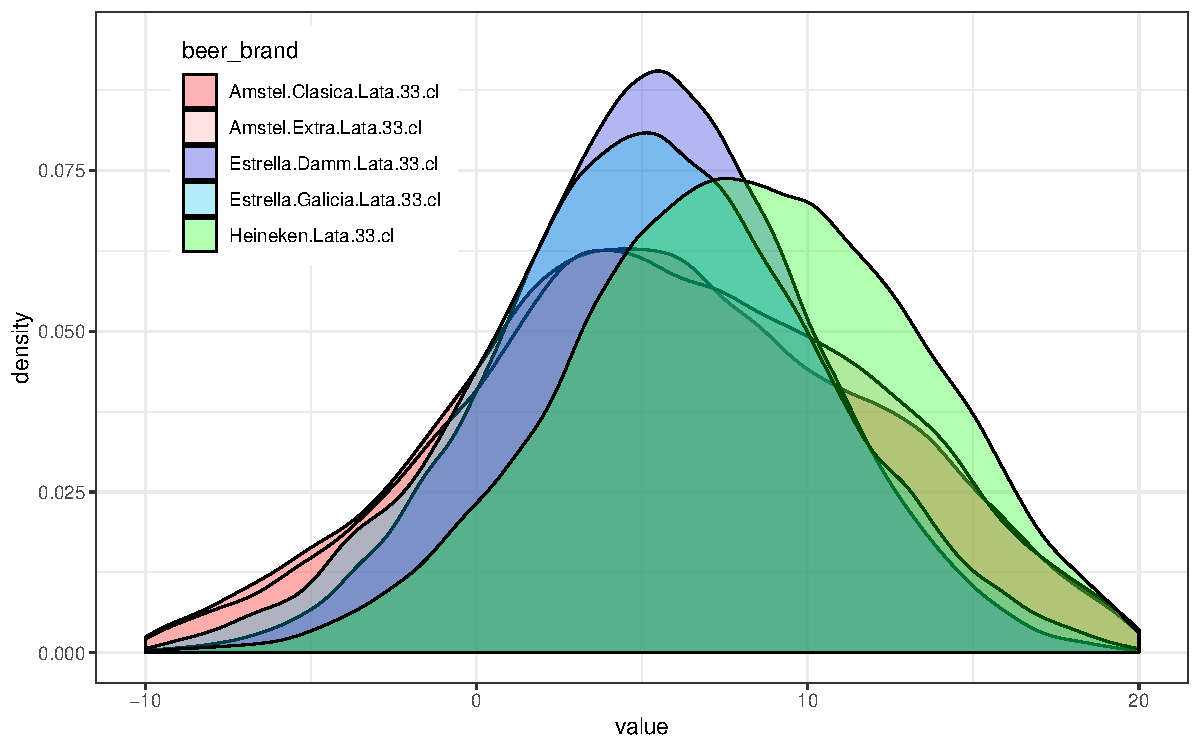
\includegraphics[scale = 0.6]{figures/dens_betas_five_in_one.pdf}
	\caption{Density plot for betas of five distinct brands}
	\label{fig_dens_five}
\end{figure}

The density plot reveals very similar preferences for both Amstel beers.
It is therefore interesting to have a look at the bivariate density plot that displays their joint beta distribution.
Figure \ref{fig_dens_amstel_biv} reveals that there is a slightly higher preference in the sample for Amstel Extra Lata compared to Amstel Clasica Lata.
This finding will subsequently explain large price discrepancies between those brands in a monopoly (see section \ref{sec_marketsim}).

\begin{figure}[ht]
	\centering
  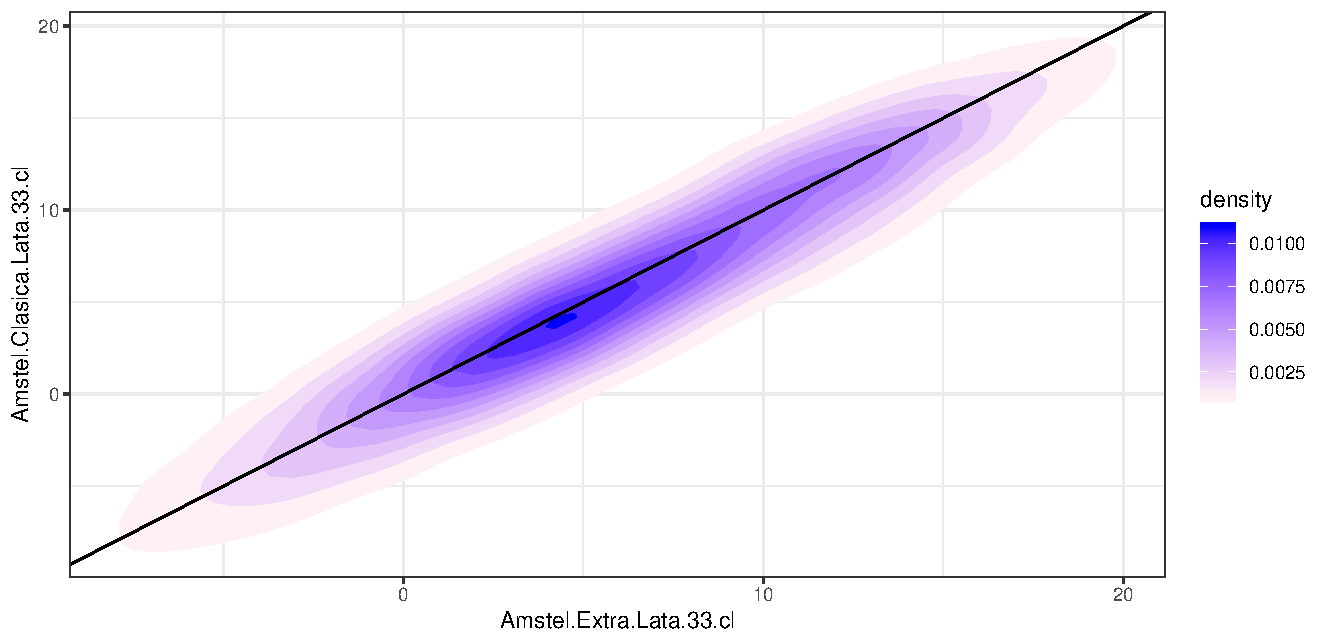
\includegraphics[scale = 0.6]{figures/amstel_bivariate_density.pdf}
	\caption{Bivariate density plot for two Amstel brands displaying slightly higher preferences for Amstel Extra Lata}
	\label{fig_dens_amstel_biv}
\end{figure}

Not only the density plots of beta distributions are of interest---their similarity in terms of correlation can quantify how similar individual brands are compared to another one.
The higher the correlation between two brands, the more similar are customers' preferences for those two beers.
Most importantly, this implicates that there is a high price-competition between those brands.
If there is a high correlation between preferences, customers regard two brands as good substitutes and therefore are mainly guided by the beer's price in their purchase decision.
Turning to the subset of beers at hand, the two Amstel brands show the highest correlation ($\rho=0.95$), followed by a correlation coefficient of 0.72 and 0.75 for the Amstel brands with Heineken.
This provides a first clue that Amstel and Heineken find themselves in a strong price competition, because they serve similar customers.
Contrary to that, a low correlation between the distribution of two beta coefficients implies that those brands compete less price-wise, since they serve different segments of the market.
Especially noteworthy is that Estrella has the least correlated beta distributions compared to all other brands, which indicates that they compete least for similar customers compared to Heineken and Amstel.

Lastly, the correlation matrix also displays the correlation of betas for beer brands with betas for price.
This is an indicator how price-sensitive customers are to price changes.
Interestingly, customers of Estrella Galicia Lata are found to be almost completely price insensitive ($\rho=0.02$), while Heineken's customers are most influenced by price changes ($\rho=0.52$).
All else equal, a price increase by Heineken will cause a greater customer churn than the same price increase for Estrella, since the latter's customers are least price sensitive and might be influenced mainly in their purchasing decision by quality rather than price.

\begin{figure}[ht]
	\centering
  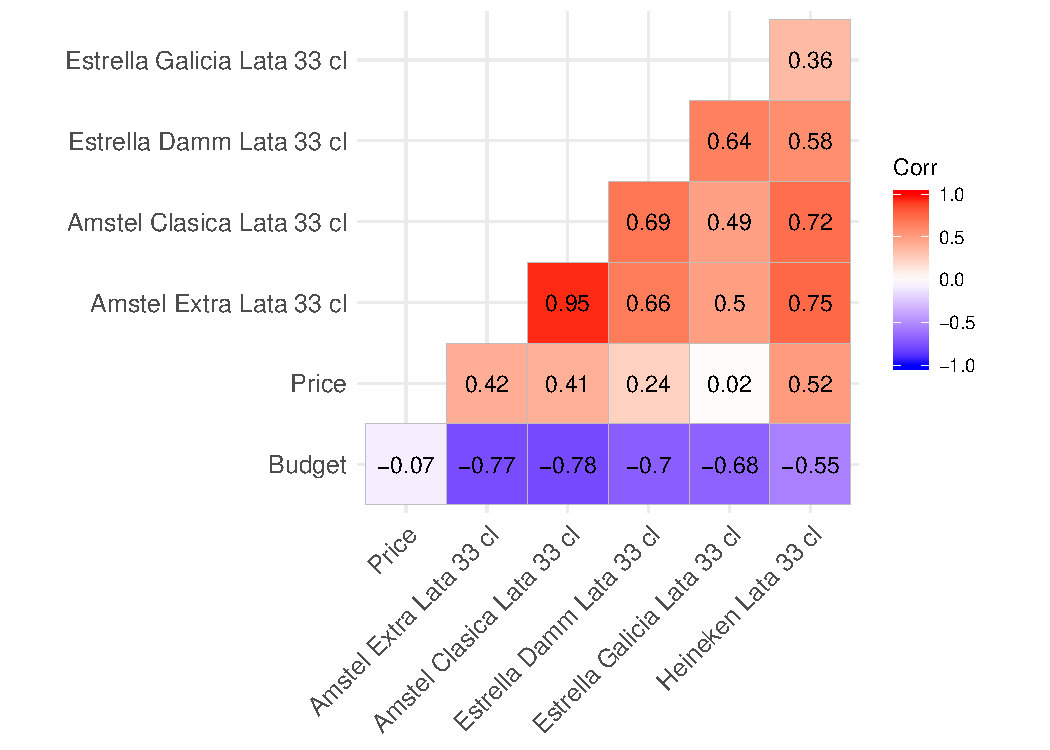
\includegraphics[scale = 0.7]{figures/corrplot_betas_five.pdf}
	\caption{Correlation of betas for price, budget and five brands}
	\label{fig_corr_five}
\end{figure}


\section{Market Simulation} \label{sec_marketsim}

However interesting the beta coefficients as measures of preferences might be, they enable managerial decisions in a limited way and provide a very technical and abstract economic interpretation in terms of preferences.
To enhance the usefulness of the hierarchical Bayesian MNL model, the resulting distributions of beta coefficients can be translated into Nash equilibrium prices, shares and profits.
This section describes the beer market simulation and its results for the relevant subset of five brands in four different scenarios from full competition to monopoly.
A focus will be set on the difference between the two scenarios in the middle: brand competition and merge competition, where the first refers to a market environment before the merger and the latter to a duopoly in which Heineken and both Amstel brands belong to the same profit-maximizing owner.

To compare the different scenarios, three metrics are calculated: First, Nash equilibrium prices $p_i$, which refer to the $i^{th}$ beer's profit optimal price.
Equilibrium price in this case means that a deviation for all players from its respective price would no longer result in a higher profit.
Based on that, the market shares $MS_i$ are computed for all brands as well as for the outside good (i.e. consumers choose to not purchase any beer).
Combining the two metrics price and market share with marginal costs\footnote{as stated in section \ref{sec_intro}, this study assumes constant marginal costs of $MC = 0.192 \text{\euro}$ across all products.} enables the calculation of the product of contribution margin and market share, which is proportional to profits\footnote{no assumption about the market size is made. A simple multiplication of the market size with the formula above would lead to profits.}:
\begin{align*}
Profit_i \propto (p_i - MC) * MS_i = CM_i * MS_i
\end{align*}
Those three metrics enable a clear overview over market outcomes on individual brand level.
However, it is also of high interest to quantify the aggregate market result, which can be achieved by computing the weighed average price in the market 
\begin{align*}
\bar{p}_m = \sum_{i=1}^n{p_i * MS_i},
\end{align*}
where $n$ refers to the number of players plus one outside good.
By including the outside share at a price of 0, this metric quantifies a trade-off between the brands' prices and the outside share.
Higher market power in the market leads to two changes that adversely affect $\bar{p}$: First, individual prices increase leading to an increase in $\bar{p}$.
Second, the outside share increases since some customers drop out of the market, which causes $\bar{p}$ to decrease.
If the weighed average price remained constant after a merger in the market, that means the increase in individual prices is compensated by the increase in the outside share.
This enables a conclusion about which effect dominates in certain situations.

\begin{figure}[ht]
	\centering
  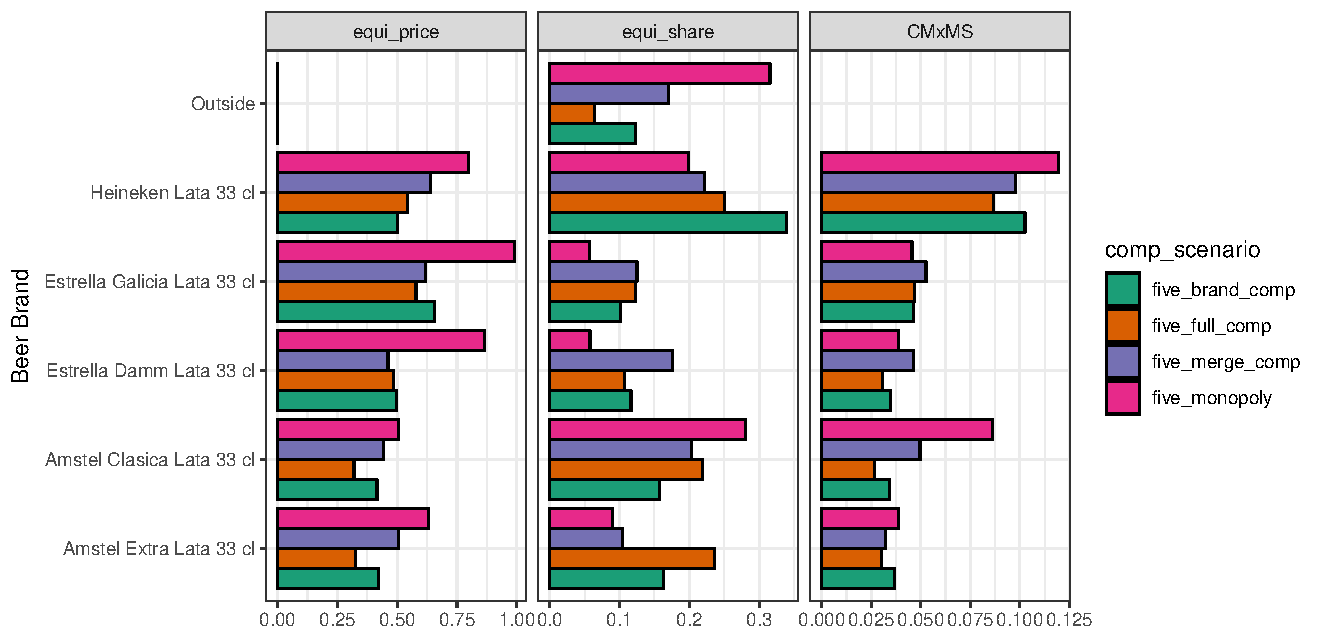
\includegraphics[scale = 0.7]{figures/bar_price_share_brand_merge_5.pdf}
	\caption{Prices and market shares in a profit-maximizing Nash equilibrium for five brands and outside option in a brand competition vs. merge setting}
	\label{fig_bar_five}
\end{figure}

Figure \ref{fig_bar_five} visualizes the market outcomes in terms of prices, market shares and profits for each of the four market scenarios.
Overall, the results appear to be in line with economic theory.
The remainder of this section discusses the individual market scenario outcomes and its implications.
Assuming full competition (i.e. all brands compete against each other), prices for most individual brands as well as $\bar{p}$ are lowest.
As expected, lowest prices come with the lowest outside share of 6.4\%.
It is interesting to note that Heineken's price is in between Amstel's (lower) and Estrella's prices (higher).
Even though it is more than 20 cents pricier than Amstel's two beers, its market share at 25\% is the highest among all beers.
This result is in line with the distribution of the model's beta coefficients.
The average consumer prefers Heineken over all other brands and Amstel is the least preferred brand, assuming constant prices.
It is therefore not surprising that even though Heineken charges higher prices than Amstel, it's market share is higher.

Now assume competition according to the beer brands, i.e. both Amstel beers, both Estrella beers, and Heineken each belong to a different owner (brand competition).
In this market of three players, weighed average prices increase from 0.406 to 0.428\euro\ despite a rise in the outside share by nearly six percentage points.
A look at the individual prices suggests that thanks to its increased market power, Amstel increases their prices to nearly match Heineken's.
Remember that the correlation between the betas of Heineken and Amstel is relatively high, which means they serve similar customer segments.
Still, Heineken's beta distribution is shifted to the right of Amstels' distributions\footnote{see figure \ref{fig_dens_amstel_biv} for the beta distribution density plots of the five beers.}, which means that consumers on average prefer Heineken over Amstel.
Since the prices of the three brands are now more similar than before, this translates to a drastic increase in Heineken's market share to more than one third of the entire market and a modest decrease in both Amstels' shares by around seven percentage points each.

\begin{table}[!htbp] \centering 
  \caption{Weighed average prices in the entire market and producer surplus for three merged brands before vs. after the merger} 
  \label{tab_merge} 
\begin{tabular}{@{\extracolsep{10pt}} lcc}
\\[-1.8ex]\hline 
\hline \\[-1.8ex] 
 & $\bar{p}\text{ (\euro)}$ & $PS_m\text{ (\euro)}$ \\
\hline \\[-1.8ex] 
\begin{tabular}[c]{@{}l@{}}Before merger\end{tabular} & 0.428 & 0.173 \\
\begin{tabular}[c]{@{}l@{}}After merger\end{tabular} & 0.442 & 0.180 \\
$\Delta$ & +0.014 & +0.007 \\
$\Delta\%$ & +3.3\% & +3.5\% \\
\hline \\[-1.8ex] 
\end{tabular}
\end{table}

The research question whether a merger between Heineken and Amstel would yield an incremental profit beyond the sum of the individual profits can now be answered by changing the ownership matrix so that those three beers now belong to the same owner and thus not price compete anymore.
This market is now a duopoly with two players (Heineken and Amstel beers vs. Estrella beers) and referred to as merge competition.
\ref{tab_merge} displays the weighed average price and the producer surplus before and after the merger and quantifies the absolute and relative difference between those two scenarios.
While $\bar{p}$ increases by 3.3\%, the producer surplus even increases by 3.5\%.
This represents the incremental profit due to the merger due to higher market concentration and less price competition with beer brands that targeted similar-preferences customers.
The sole competitor Estrella's relative market power compared to the new Amstel--Heineken firm decreases.
Nevertheless, thanks to the consolidation its absolute market power increases.
Though their prices remain relatively constant, their profits increase due to a higher market share.
This is counter-intuitive at first---but has a logical explanation.
Looking at the distribution of beta coefficients in figure \ref{fig_dens_five} one can infer that preferences are higher for Estrella than for Amstel, on average.
As Amstel's prices in this scenario approach Estrella's, the latter becomes more attractive and leads to higher market shares and profits for both Estrella beers.
In line with expectations, the outside share further increases to 17\% in the duopoly.

While the first scenario represented one extreme market constellation---full competition---the last one scrutinizes the other extreme---a monopoly.
As expected, all individual prices increase and are highest among all four scenarios.
This translates in a weighed average price of 0.46\euro\, even though almost one third of the consumers drop out of the market.
Interestingly, while all individual prices increase, the individual profits do not increase by the same magnitude due to a significant decrease in market share for most brands.
Notably, the cheapest beer in this scenario is one exception to that.
Amstel Clasica Lata at $p=0.50\text{\euro}$ increases its profits by almost 75\% compared to the duopoly, while Amstel Extra Lata's profits only increase marginally.
This can be explained by the slightly higher preference of the average consumer for Amstel's Extra Lata beer over Clasica Lata visualized in figure \ref{fig_dens_amstel_biv}.
Since there is no competition anymore, the firm uses this slight preference for Extra Lata and exploits the consumers' higher willingness to pay for the more preferable beer, while the remaining Amstel brand captures all consumers that would otherwise have dropped out of the market.


\begin{figure}[ht]
	\centering
  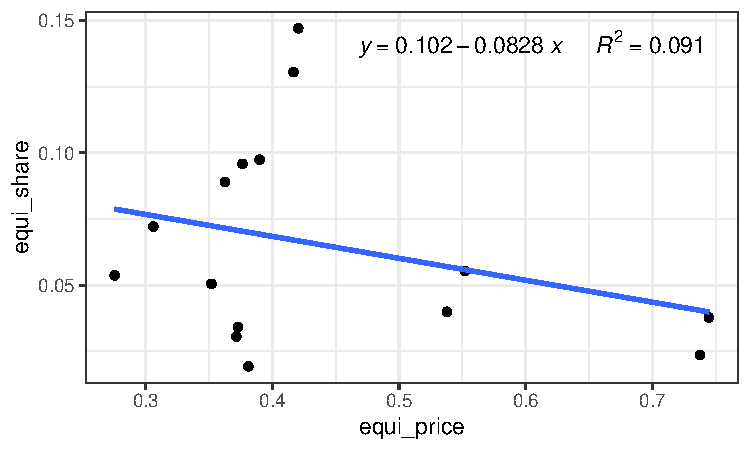
\includegraphics[scale = 0.7]{figures/scatter_price_share_brand_comp_fitted.pdf}
	\caption{Price--Market Share scatter plot with linear regression model fit}
	\label{fig_scatter_brand_comp}
\end{figure}

\section{Managerial and Research Implications}


\clearpage
\appendix
\section{Appendix}

\begin{figure}[ht]
	\centering
  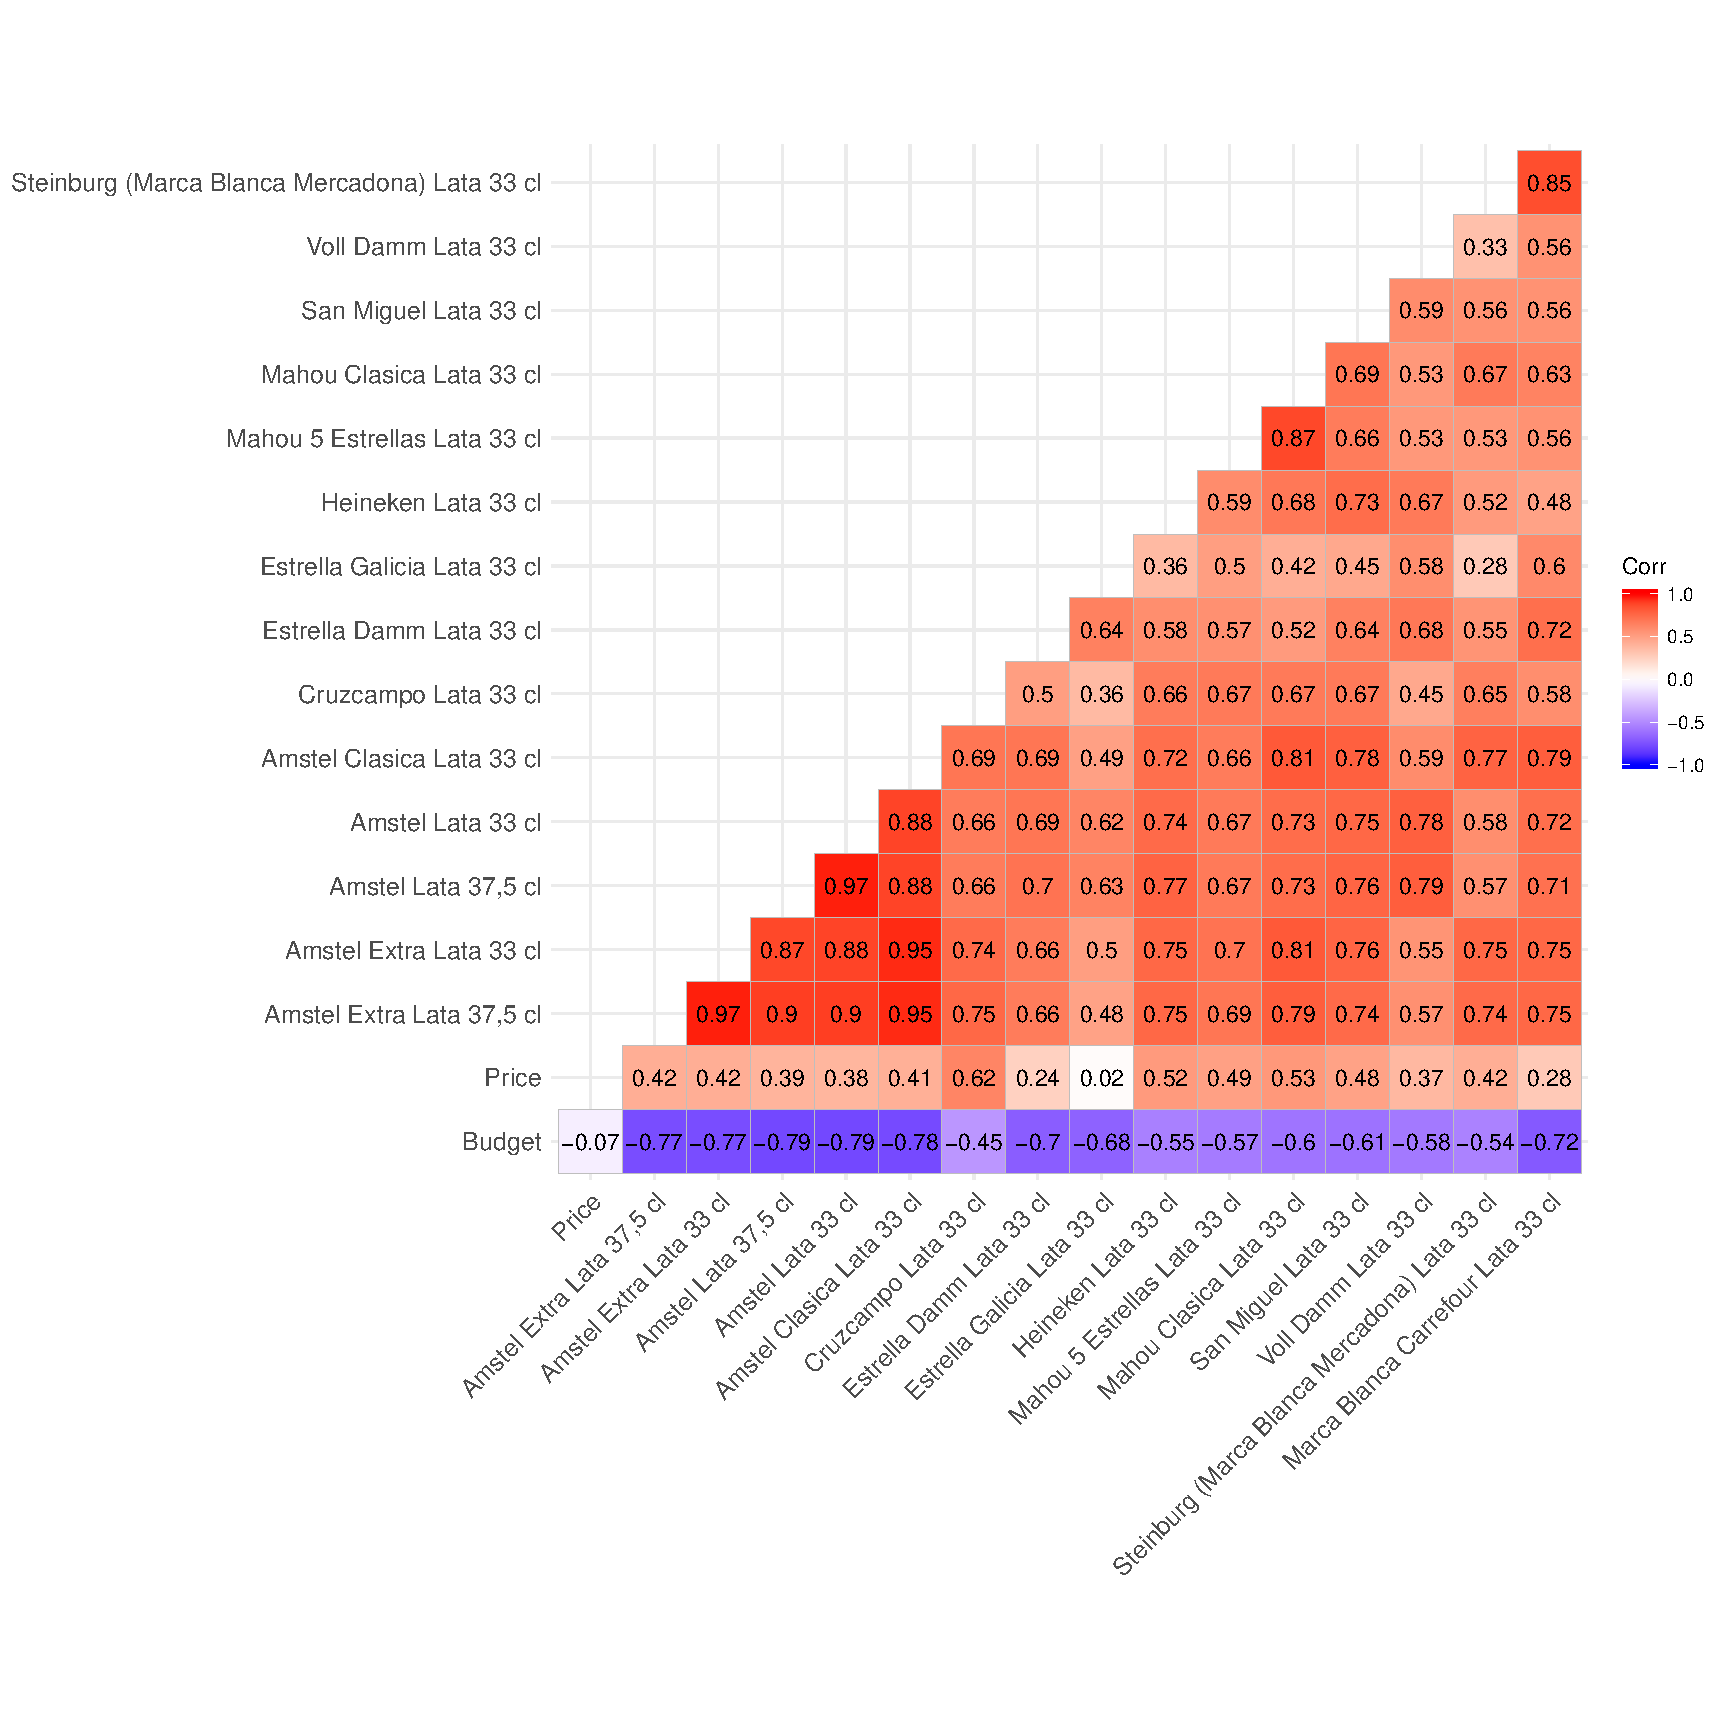
\includegraphics[scale = 0.5]{figures/corrplot_betas_full.pdf}
	\caption{Correlation of betas for price, budget and all 15 brands}
	\label{fig_corr_all}
\end{figure}

\begin{figure}[ht]
	\centering
  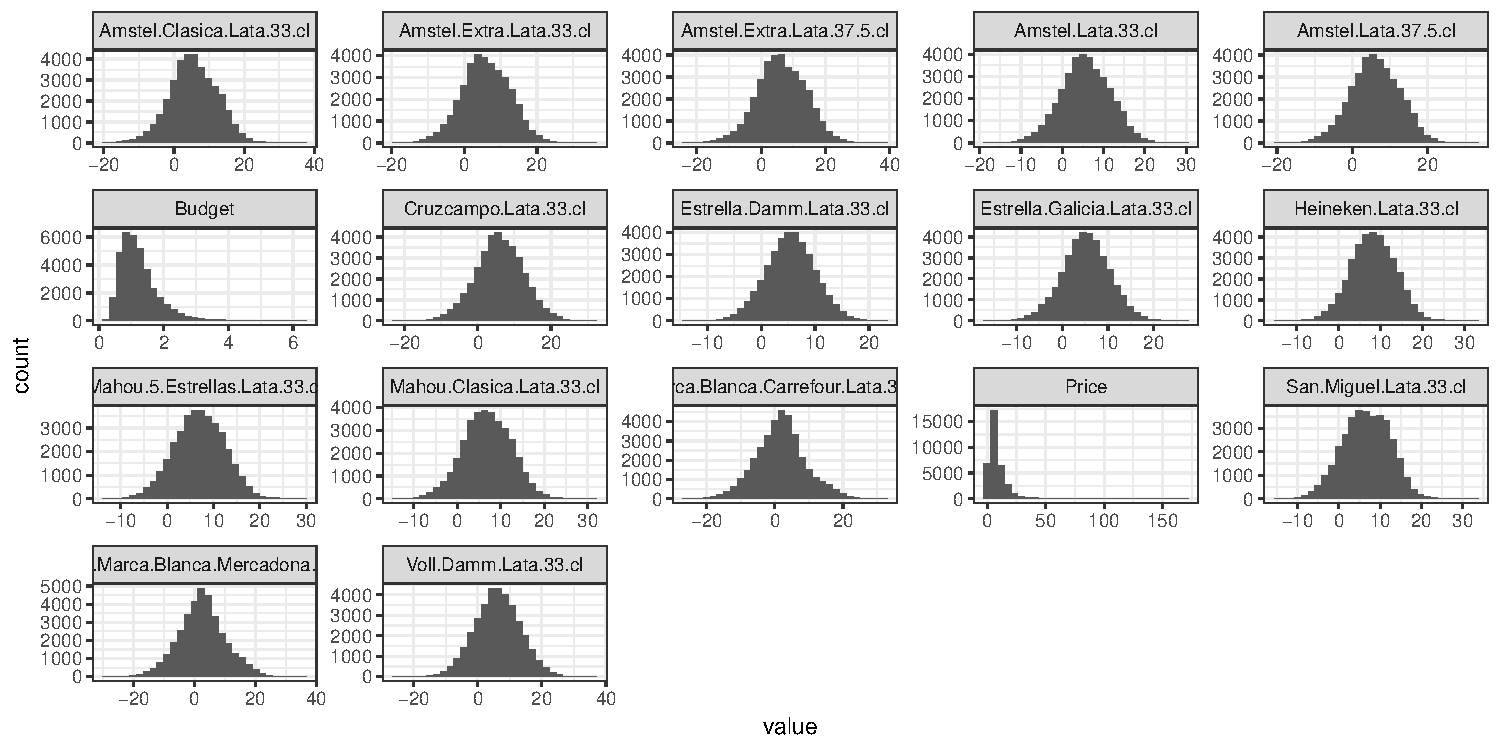
\includegraphics[scale = 0.6]{figures/hist_betas_full.pdf}
	\caption{Histograms of betas for price, budget and all 15 brands}
	\label{fig_hist_all}
\end{figure}

\begin{figure}[ht]
	\centering
  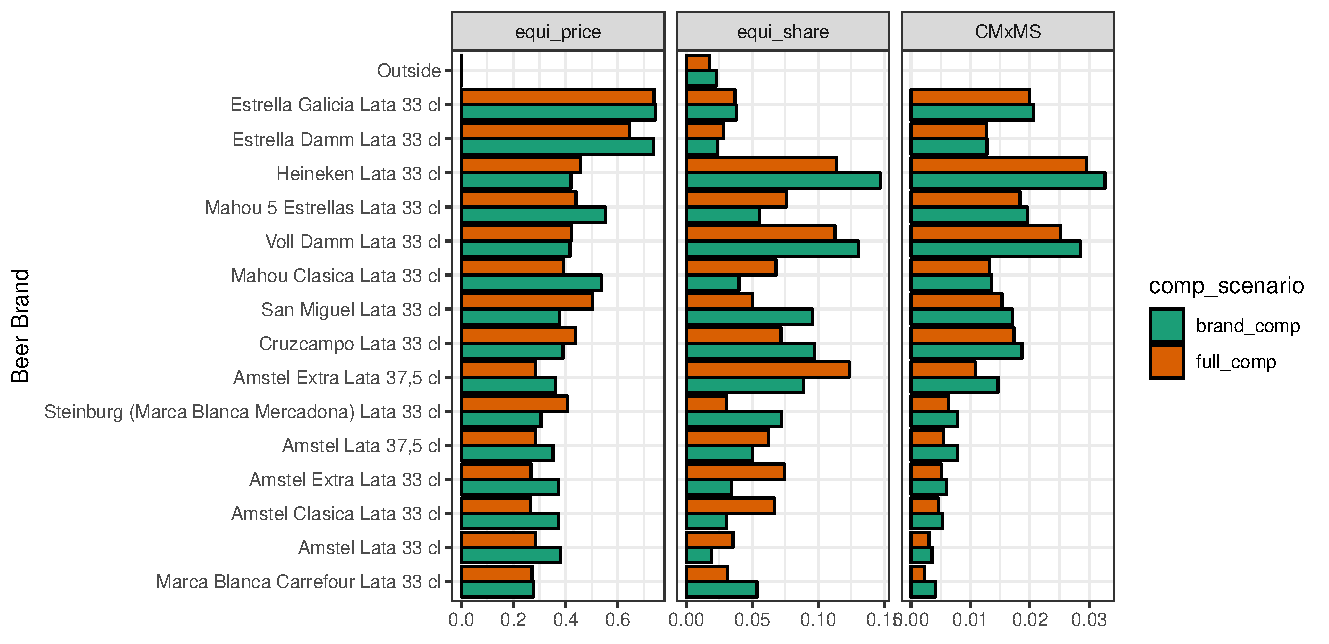
\includegraphics[scale = 0.7]{figures/bar_price_share_full_brand_15.pdf}
	\caption{Prices and market shares in a profit-maximizing Nash equilibrium for all 15 brands and outside option in a full vs. brand competition setting}
	\label{fig_bar_fifteen}
\end{figure}



\section{R Code}

%\begin{lstlisting}[language=R,caption={Estimation Code}, label=lst:estim]
%
%
%\end{lstlisting}


\clearpage
\bibliography{library}

\newpage
\thispagestyle{empty}
\section*{Statutory Declaration}

I herewith declare that I have completed the present term paper independently, without making use of
other than the specified literature and aids. Sentences or parts of sentences quoted literally are
marked as quotations; identification of other references with regard to the statement and scope of
the work is quoted. The thesis in this form or in any other form has not been submitted to an examination body and has not been published.
This thesis has not been used, either in whole or part, for another examination achievement.

\vspace{1cm}

Frankfurt am Main, July 23, 2019

\includegraphics[scale=0.12]{signature.png}\\
Lukas J\"urgensmeier
\end{document}
